\subsection{Projekt zum Schutz der Biodiversität in Rumänien}

%Einordnung meiner Arbeit in Relation zum Projekt??? -> Testflüge erwähnen, Zeitrahmen erwähnen???
Das Projekt zum Schutz der Biodiversität in Rumänien ist eine bilaterale Zusammenarbeit im Apuseni-Gebirge zum Erhalt des oligothrophen Grünlandes und insbesondere der Zielart Arnica montana. In zwei Ansätzen soll unter dem Einsatz von moderner Fernerkundungstechnologien einerseits brachliegende Flächen und andererseits Grasland mit Arnica montana erkannt werden. Mit den Erkenntnissen soll auf brachliegenden Probeflächen mit Mäh- und Mulchmaschinen ein Wiesenmanagement stattfinden. Durch die Verwendung von Drohnen sollen bisher unbekannte Flächen mit Arnica montana identifiziert werden, um so mit einer nachhaltigen Arnika-Ernte und Bewirtschaftung die Biodiversität zu erhalten. Das Projekt möchte sich in der Region für Nachhaltigkeit und Naturschutz einsetzten, unter Steigerung des Wohlergehens der lokalen Bevölkerung. Der Projektzeitplan sieht einen Start ab dem Frühjahr 2019 vor und das Projekt soll über einen Zeitraum von drei Jahren laufen. Jährlich im Juni/Juli sollen die Drohnenflüge zur Identifizierung von Arnika stattfinden. Im September/Oktober werden die Grasland-Flächen beflogen, um eine Bewirtschaftung oder das brachliegen festzustellen. Zur Vorbereitung auf die Datenerhebungen in Rumänien fanden im Juli 2018 Drohnenflüge zu Testzwecken im Schwarzwald statt.

\subsubsection{Projektpartner}
Das Projekt ist eine Zusammenarbeit der Albert-Ludwigs-Universität Freiburg (ALU-FR) mit dem rumänischen Unternehmen Bioflora Apuseni (BFA) und der Universität für Agrarwissenschaften und Tiermedizin Cluj-Napoca (USAMV). Die ALU-FR wird vertreten durch Prof. Dr. Dr. h.c. Albert Reif (Proffessur für Standort- und Vegetationskunde), Dr. Evelyn Ruşdea  (Projektmanagement) und durch Dr. Holger Weinacker (Institut für Fernerkundung und Landschaftsinformationssysteme). Die ALU-FR hat stellvertretend für das Projekt einen Finanzierungsantrag bei der Deutschen Bundesstiftung Umwelt gestellt.

Das Unternehmen Bioflora Apuseni (BFA) wurde 2010, nach einem langen Prozess der deutsch-rumänischen Zusammenarbeit und Forschung, gegründet. BFA hat es sich zum Ziel gesetzt die ländlichen Bevölkerung im Zentrum des Apuseni Gebirges im nachhaltigen Umgang mit natürlichen Ressourcen zu unterstützten, um die artenreiche Kulturlandschaft der oligotrophen Graslandes zu erhalten und den Lebensstandard zu erhöhen. Das Hauptprodukt ist Arnica montana, welches von den rund 25 SaisonarbeiterInnen von BFA nachhaltig gesammelt und dann in einer lokalen Trocknungsanlage getrocknet. Hauptabnehmer zu einem fairen Preis ist Weleda, die auch gemeinsam mit BFA regelmäßige Schulungen für lokale PflückerInnen organisieren, um die nachhaltige Ernte der Arnikablüten sicherzustellen. Es gibt Entwicklungen? weitere Heilpflanzen zu vermarkten und neue Abnehmer zu finden. Außerdem initiert BFA weitere Pilotprojekte in anderen Regionen Rumäniens, damit auch dort Arnika nachhaltig geerntet werden kann \citep[vgl.][]{ECOKARST2018,DBU2018}.

Die Universität in Cluj-Napoca (USAMV) erforscht seit 2000 im Apuseni Gebirge die traditionelle Bewirtschaftung des Graslandes, um das Management zu optimieren und zu erhalten. Es gibt unter anderem eine Langzeitstudie zu den Folgen von Düngern auf die Biodiversität des Graslandes im Apuseni Gebirge. Als assoziierter Partner wird der Drohnen-Pilot und Videoeditor Paul Crişan für das Projekt an der USAMV angestellt. Weitere assoziierte Partner sind der Naturpark Apuseni, die LEADER-Initiative (GAL Arieşul Mare) sowie die Firma Weleda.

Bereits von 2000 bis 2004 gab es eine erste Zusammenarbeit der ALU-FR mit der rumänischen USAMV mit dem gemeinsamen „Projekt Apuseni“, aus dem die Identifizierung von Arnica montana im Zentrum des Apuseni Gebirges hervorging. Finanziert durch das Bundesministerium für Bildung und Forschung (BMBF) wurden sieben kleinere Pilotprojekte in verschiedenen Bereichen, wie ländlichem Tourismus, Landwirtschaft, Wasserversorgung, Arzneipflanzen und Waldwirtschaft durchgeführt. Dabei wurde bewusst ein partizipativer Ansatz (buttom-up) gewählt, da vor Ort die Landschaft Allgemeingut ist, das von vielen Menschen beansprucht wird. Deshalb wurden auch möglichst viele Personen in den Prozess der Entwicklung eines nachhaltigen Landschaftmanagements involviert. Neben Interviews mit LandwirtInnen, ExpertInnen und lokalen PolitikerInnen wurden Treffen, Workshops und  Vorträge organisiert, Informationsmaterialien verteilt, Beratungen und Rollenspiel durchgeführt und ein Schul-Projekt „Planning for real“ angeboten. Darin bauten die SchülerInnen gemeinsam ein dreidimensionales Model des Dorfes, wie es in 15 Jahren aussehen soll. Aus den Projekten ließen sich die Stärken und Schwächen der Bergregion herausfiltern, um damit Empfehlungen für die regionale Entwicklung zu formulieren? \citep[vgl.][]{RUSDEA2009}.
Im Anschluss startete ein weiteres Projekt, diesmal mit dem Schwerpunkt auf \textit{Arnica montana}, 2004 im Apuseni Gebirge. Das „Arnika Projekt“ lief bis 2007 und wurde vom World Wide Fund For Nature (WWF) und der Darwin Foundation is Zusammenarbeit mit der USAMV durchgeführt. Im Ausbau der Kooperation mit der lokalen Bevölkerung wurde der Kontakt zu BesitzerInnen von oligotrophen Wiesen und potenziellen Arnika PflückerInnen hergestellt. Durch Interviews wurde die traditionelle Bewirtschaftung der oligotrophen Wiesen erforscht und Trainings zur nachhaltigen Ernte der Blütenstände der \textit{Arnica montana} durchgeführt \citep[vgl.][20]{DBU2018}.

\begin{figure}[htb]
 \centering
 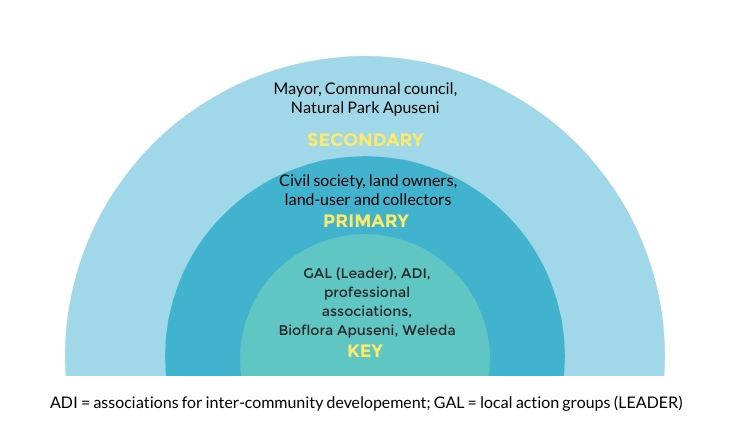
\includegraphics[width=0.7\textwidth,angle=0]{abb/Stakeholder-map}
 \caption{Stakeholder map \citep[nach][]{DBU2018}}
\label{fig:stakeholdermap}
\end{figure}

%Stakeholder map erklären:
Im Projekt wird zwischen Key Stakeholder, primären und sekundären Stakeholdern unterschieden (Siehe Abbildung~\ref{fig:stakeholdermap}, S.\pageref{fig:stakeholdermap}). Die etablierten Organisationen, wie BFA, Weleda und die lokale Aktionsgruppe (LAG/GAL) Arieşul Mare und die Associations for inter-community development (ADI) sind aufgrund von ihrer Erfahrung im Naturschutz vor Ort die Key Stakeholder. Primärer Stakeholder ist die ansässige Bevölkerung, insbesondere die EigentümerInnen oder PächterInnen der Flächen oder SammlerInnen der Wildkräuter. Als sekundäre Stakeholder bilden die die administrativen Stellen in der lokalen und regionalen Behörden und die Verwaltung des Naturparks Apuseni.

\subsubsection{Ökologischer Hintergrund}

Das Apuseni Gebirge befindet sich im nordwestlichen Teil von Siebenbürgen in Rumänien. Es bildet den nördlichen Teil der Rumänischen Westkarpaten und erreicht Gipfelhöhen von 1100 bis 1800 m. Die Landschaft ist geprägt durch Steilhänge und Karstformen, wie Dolinen, Polje, Trockentälern, Karsttreppen und Unterirdischen Höhlen. Die Region hat eine geringe Einwohnerdichte, aber die höchste Einwohnerdichte im Vergleich zu anderen Bergregionen Rumäniens. Vor einer Besiedelung gab es ursprünglich nur Waldgebiet mit Kiefer und Buchen. Durch die Nutzung der Ressource Holz entstand das Grasland von heute. Die Landnutzung beträgt heute noch ca. 55\% Wald (davon ca. 79\% Laubwald, 12,34\% Nadelwald und 3,5\% Mischwald, rest ist Übergangsvegetation), 17,4\% Grasland, 3,09\% Brachland, 1,84\% Besiedelung und 0,61\% Ackerland (Gärten).

Vor 1989 war die Waldwirtschaft in Rumänien streng geregelt und kontrolliert. In der Zeit danach nahm die Abholzung? im Apuseni Gebirge stetig zu, weil der kommerzielle Wert von Holz auf dem europäiischen Markt erkannt wurde. Dies führte zum drastischen Rückgang der Wälder im Apuseni-Gebirge, insbesondere von Nadelbäumen. Die derzeitige Regierung versucht dem entgegen zu wirken und hat neue Regelungen erlassen, nach denen pro Person nur 20m\textsuperscript{3} Holz im Jahr gefällt werden dürfen. Größere Unternehmen sind davon ausgenommen, was einen Nachteil für die lokalen Bevölkerung darstellt, die ihre Haupteinnahmequelle, die Holzverarbeitung und Aufwertung, verliert. Eine signifikante Abwanderung ist die Folge, was auch einen negativen Effekt auf das Management von Grasland hat.

Das oligotrophe Grasland kann seine Biodiversität nur erhalten, wenn eine Bewirtschaftung stattfindet. Das Brachliegen oder die Intensivierung der Nutzung gefährdet das schwierige Gleichgewicht der Graslandwiesen. Zum Schutz der Biodiversität muss eine gemäßigte Düngung von biologischen Düngern (keine Mineraldüngung!) periodisch aufgetragen werden. Um optimale Bedingungen für eine hohe Vielfalt an Arznei- und Wildpflanzen zu erhalten, müssen die Flächen etwa jährlich gemäht werden und dazwischen geflegt werden, z.B. durch das Entfernen von Ästen und Steinen.

\todo{hier muss noch zu dem tatsächlichen Manangement recherchiert werden}

\subsubsection{Vorgehensweise}

Zur Identifikation von brachliegendem oligotrophen Grasland sollen mit dem Einsatz von Drohnen Digitale Höhenmodelle erstellt werden. Dafür muss das gesamte Gelände zweimal mit der Drohne erfasst werden. Beim ersten Flug wird ein Digitales Oberflächen Modell (DOM) (engl. digital surface model DSM) erstellt, also ein Modell der Erdoberfläche inklusive auf ihr befindlicher Objekte, wie die Vegetation. Nach dem zweiten Flug kann ein Digitales Geländemodell (DGM) (engl. digital terrain model DTM) abgeleitet werden. Das DGM ist ein Modell der natürlichen Erdoberfläche ohne Objekte. Durch die Subtraktion der beiden Modelle kann ermittelt werden, ob Flächen gemäht wurden oder ob sie brachliegen. Nach der Indentifikation von brachliegenden Flächen werden fünf Probeflächen in fünf Gemeinden ausgewählt und durch den Einsatz von Mäh- und Mulchmaschinen wieder nutzbar gemacht. In Zusammenarbeit mit der lokalen Aktionsgruppe Arieşul Mare soll der Kontakt zwischen LandbesitzerInnen initiiert werden. Mit dem Zusammenschluss gibt es die Perspektive weitere Technologien und Maschinen anschaffen zu können und das Projekt auf andere Regionen ausweiten zu können.

Mit der nachhaltigen Vermarktung von Arnica montana soll in die Bevölkerung ein Interesse zum Schutz des oligotrophen Graslandes geschaffen werden. Durch die Verknüpfung der ökonomischen Interessen mit dem ökologischen Erhalt der Biodiversität soll langfristig eine Steigerung der Lebensqualität der vor Ort lebenden Menschen erreicht werden. An die Entwicklung der BFA soll hier angeschlossen werden. Ziel ist es eine Datenbank und Karte über die Verteilung der Arnika-Flächen in zehn Gemeinden zu erstellen. Durch den Einsatz von Drohnen in fünf Gemeinden soll das Produktivitätspotential der Habitate ermittelt und in eine qualitative Klasse in Abhängigkeit von der Anzahl der Blütenstände pro 100 m\textsuperscript{2} eingeordnet werden. Zusätzlich soll erfasst werden, welches Management bisher auf den Flächen durchgeführt wurde. Für die Auswertung der durch den Drohneneinsatz entstandenen Bilder soll ein Software-Programm entwickelt werden, dass die Arnica montana Blütenstände automatisch erkennt und eine Klassifizierung durchführt.

\subsubsection{Drohneneinsatz zur Fernerkundung}

%+++ Was ist eine Drohne? Was eine UAS, UAV?
Drohnen sind Luftfahrzeuge, die ohne an Bord befindliche Personen über einen Computer oder vom Boden aus über eine Fernsteuerung betrieben werden. Unbemannte Luftfahrzeuge (engl. Unmanned Aerial Vehicle, kurz UAV) besitzen zwei Tragflächen und sind dem Flugzeug nachempfunden. Multikopter zählen zu den Hubschraubern und haben zwischen zwei und zwölf Rotoren, so können sie sich in alle Richtungen bewegen. Beide werden im allgemeinen Sprachgebrauch Drohnen genannt. Ferngesteuerte Fluggeräte, die im Freizeitbereich eingesetzt werden, zählen nicht zu den Drohnen, auch wenn vor allem die Multikopter Flugmodelle oft so bezeichnet werden. Unmanned Aerial Systems (UAS) bestehen aus der UAV, der Sensor-Ladung und der Bodenkontrollstation. Komponenten und Größe der Bodenkontrollstationen variieren stark, in Abhängigkeit von der Aufgabe der UAV. Sie können aus großen Kontrollsystemen bestehen, die auf Fahrzeugen montiert werden oder nur aus einem kleinen Laptop, der getragen werden kann. \citep[vgl.][]{Watts2012}
%Die Klassifizierung von UAS im zivilen wissenschaftlichen Einsatz orientiert sich generell auf den schon vorhandenen militärischen Begriffen. Die Einteilung basiert auf den Eigenschaften Größe, Flugausdauer und weiteren Fähigkeiten der Drohnen.
\begin{figure}[hbt]
    \subfigure{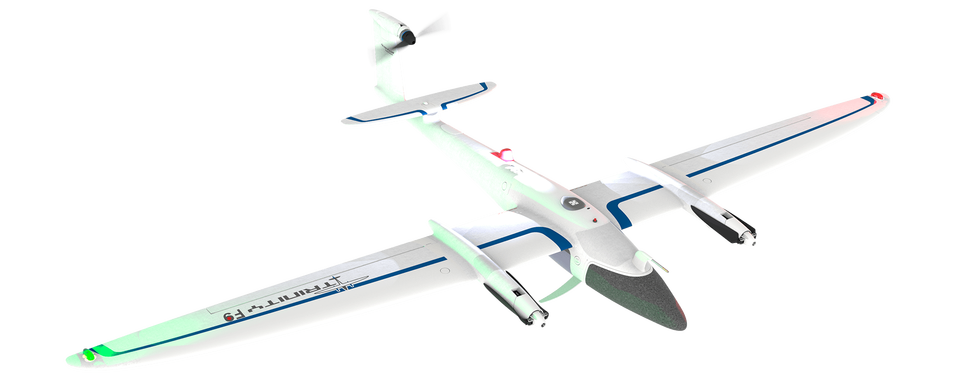
\includegraphics[width=0.65\textwidth,angle=0]{abb/drohnen/trinity-f9}}
    \subfigure{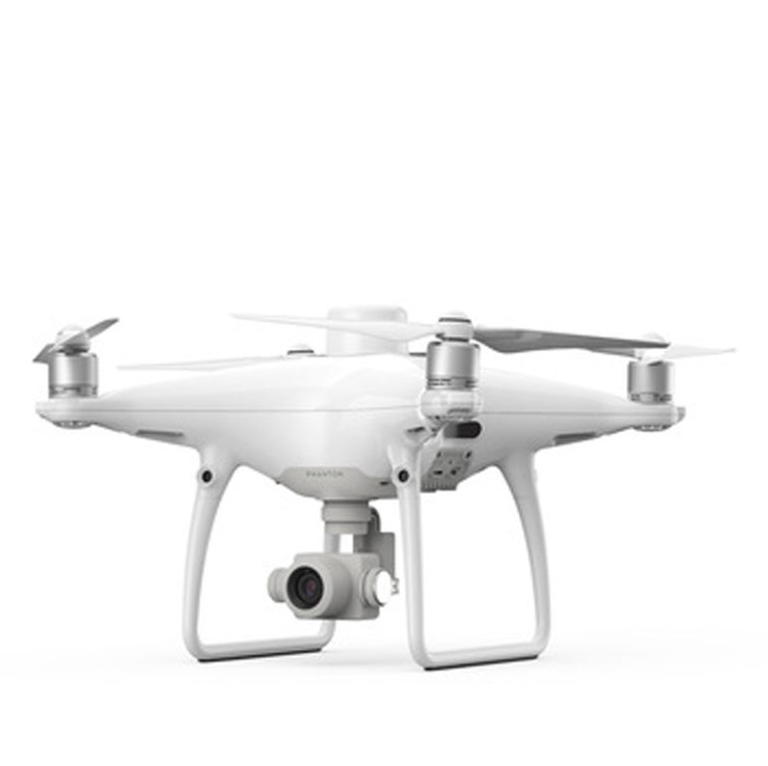
\includegraphics[width=0.3\textwidth]{abb/drohnen/P4RTK}}
\caption{Trinity F9 VTOL-Drohne (links) und DJI Phantom 4 Quadrocopter (rechts)}
  \label{fig:drohnen}
\end{figure}

Für den Anwendungsmaßstab des Projekts in Rumänien sind zwei Arten von Drohnen geeignet (Siehe Abbildung~\ref{fig:drohnen}, S.\pageref{fig:drohnen}). Die Multikopterdrohnen können präzise Aufnahmen in einer angemessene Höhe machen, haben durch den Schwebflug aber einen höheren Energieverbrauch und somit eine kürzere Flugdauer. „Vertical Take-Off and Landing“ (VTOL) Drohnen sind UAV, die keine Start- oder Landebahn benötigen. Durch ihre Tragfläche können VTOL Drohnen eine große Fläche in geringer Zeit befliegen. Zum Starten und Laden haben sie Rotoren, die nach oben gerichtet werden. Dadurch sind sie auch in unwegsamen Gelände einsetzbar.

Generell stehen die mögliche Flugzeit und damit auch die Größe der Fläche, die von der Drohne erfasst werden kann, in Abhängigkeit zum Gewicht der Drohne. Eine höhere Beladung, durch weitere Sensoren, beispielsweise eine Kamera mit einem größerem und schwerem Objektiv, bringen genauere Ergebnisse, aber verkürzen durch ihr Gewicht die mögliche Flugzeit. Einen großen Teil des Gewichts macht aber auch der Akku aus, dessen Größe sich aber auch positiv auf die Flugdauer auswirkt.

Das „Projekt zum Schutz der Biodiversität in Rumänien“ behandelt zwei Aufgaben, die unterschiedliche Anforderungungen an eine Drohne stellen. Bei der Befliegung des Graslandes zur Erkennung von brachliegenden Flächen ist eine riesige Fläche zu erfassen. Eine UAV mit Starrflügeln kann im Vergleich zu Multikoptern höher fliegen und hat somit eine größere Flugausdauer, so kann eine größere Fläche abdeckt werden. Mit einer „Vertical Take Off and Landing“ Drohne (VTOL) können Schäden beim Start oder Ladung in unebenen Gelände vermieden werden. Da die Vegetation des Graslandes nur eine Höhe von 20-30 cm hat, muss zur genauen Berechnung der Höhenmodelle die möglichst genaue vertikale und horizontale Position der Drohne erfasst werden. Dementsprechend wird ein System  benötigt, dass die Ungenauigkeiten der globalen Navigationssysteme (GNSS), die üblicherweise ein paar Meter betragen, ausgleicht. Mit real-time kinematics (RTK) und post-processing kinematics (PPK) Systemen kann eine genaue Positionsbestimmung bis auf wenige Zentimeter berechnet werden. Wie der Name schon sagt, findet diese Berechnung beim RTK in unmittelbar statt, beim PPK nachgelagert. 

Der Vorteil von RTK und PPK ist, dass die Verwendung von Bodenreferenzpunkten entfällt, was Kosten spart. Für Beide wird eine GNSS-Bodenstation benötigt, die georeferenziert ist, um ein genaues Ergebnis zu erzielen. Bei PPK kann auch falls vorhanden mit einer virtuellen Referenzstation gearbeitet werden. 

Bei RTK muss eine Verbindung zwischen Drohne und GNSS-Bodenstation vorhanden sein, bei Störungen kann ein genaues Ergebnis nicht berechnet werden. Bei PPK ist eine Verbindung nicht notwendig, die genaue Positionierung wird erst bei Auswertung der Log-Daten berechnet. 



Für die Identifizierung von 5-8 cm großen Arnika-Blüten benötigt man hingegen eine Drohne, die Bilder in einer möglichst hohen Auflösung machen kann. Da Starrflügel UAVs eine höhere Mindestgeschwindigkeit haben als Multikopter, die auch in der Luft „stehen“ können, könnte sich die Fluggeschwindigkeit negativ auf die Qualität der Bilder auswirken. 

Einerseits die großflächige Identifizierung von neuen Flächen oligothrophen Grünlands mit dem Einsatz von Drohnen und damit einhergehend die Etablierung eines Monitorings für die nachhaltige Nutzung von Arnica montana.



task b.
hier ist es wichtig tiefer Flughöhe mit der langsamsten Geschwindigkeit -> deshalb FixWing UAV
dann können wir sicher gehen, dass die Auflösung der bilder hoch genug ist, um das best möglichste ergebnis des logarithmus zu bekommen
also muss die niedrigste Flughöhe gewählt werden, ohne aber in höhere Objekte wie Bäume zu fliegen, Weil eine FixWing UAV aber nicht langsamer als 16m/sec fliegen kann, ist eine sehr gute Kamera nötig mit einem sehr lichtempfindlichen Objektiv (z.B. Sony RX1RII)

-> Ideal wäre eine Drohne für die "Fern"-erkundung und eine für die Qualitative präzisere Erkennung. De facto wird im DBU-Antrag aber nur eine Drohne vorgeschlagen, wegen des Budgets. -> WingtraOne mit PPK

Kamera mit Auflösung zwischen 0,7 und 31 cm !!! -> tatsächlich für die Qualitative Erkennung von Arnica sehr schwierig. -> Test mit Bild aus 80m Flughöhe machen für die Diskussion

\begin{table}[htbp]
\fontfamily{cmss}\selectfont
\small
\begin{tabular}{lccc} %\toprule
\textbf{Technische Daten} & \textbf{DJI Phantom 4 RTK} & \textbf{Trinity F9}  & \textbf{WingtraOne} \\ %\midrule
\hline\hline
Flügelbreite & 0,35 m & 2,394 m & 1,25 m \\
Max. Fluggeschwindigkeit & 50 – 58 km/h & 60 km/h & 57,6 km/h \\
Max. Flugzeit & 30 min & 60 min & 55 min \\
Windwiderstand am Boden & 10 m/s & 7 m/s & 8 m/s \\
Windwiderstand im Flug & 10 m/s & 12 m/s & 12 m/s \\
Max. Fläche & 100 ha (182 m) & 500 ha (100 m) & 320 ha (120 m) \\
Auflösung & 1,5 cm/px (120 m) & 2,5 cm/px (100 m) & 2,8 cm/px (120 m) \\
Max. Startgewicht & 1,391 kg & 4,5 kg & 4,5 kg \\
max. Zuladung & – & 550 g & 800 g \\
Sensoren & RTK und Gimbal\textsuperscript{1} & PKK & PKK \\
Positionierungsgenauigkeit\textsuperscript{2} &  & 2 – 5 cm &  \\
{    } vertikal & 1,5 cm + 1 ppm RMS &  & 2 cm  \\
{    } horizontal & 1 cm + 1 ppm RMS &  & 1 cm + 0,003\% RMS\\
Preis & 7.800 EUR & 14.850 EUR & 36.678 EUR\\
\hline
\end{tabular}
\scriptsize
1: Gimbal ist ein Bildstabilisator \\
2: RMS = Root Mean Square entspricht der Standardabweichung \\
1 ppm = pro km nimmt Wertgenauigkeit um 1 mm ab. 
\caption[Tabelle]{Technische Daten der Drohnen im Vergleich}
\label{tab:technischedaten}
\end{table}

\todo{es fehlt die minimale Geschwindigkeit}
%+++ Warum diese Drohne bei dem Projekt? (Diskussion??)


\begin{figure}[htb]
 \centering
  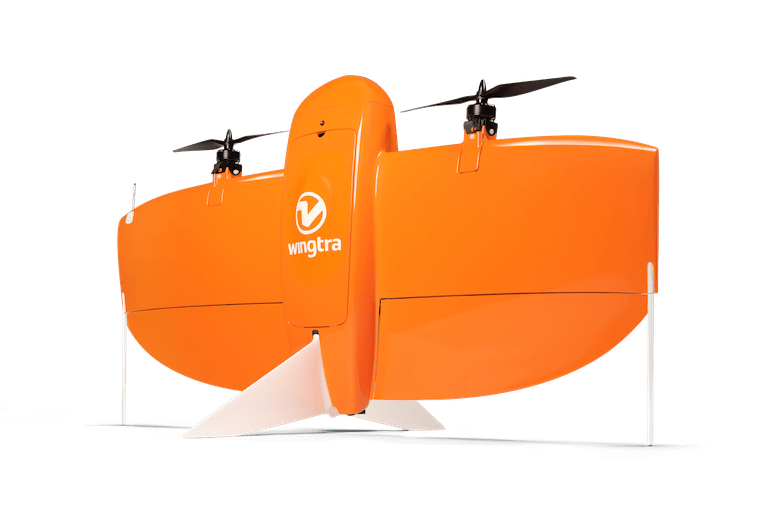
\includegraphics[width=0.6\textwidth,angle=0]{abb/drohnen/wingtraone}
 \caption{WingtraOne VTOL-Drohne}
\label{fig:wingtraone}
\end{figure}
%%%%%

\subsubsection{Testflüge im Schwarzwald}
%++++++ Testflüge?? im Schwarzwald 

Bei Testflügen im Schwarzwald im Juli 2018 wurden erste Bilder an einem bekannter Standort von Arnica montana gemacht. Mit der Octocopterdrohne der Universität Freiburg wurden mit einer Sony Alpha 7R Kamera eine Fläche in unterschiedlichen Flughöhen erfasst. Anschließend wurden die Daten ausgewertet, Höhenmodelle berechnet und Orthofotos erstellt. Ziel war es mit den Testflügen den Bedarf und Beschaffenheit der Ausrüstung für die spezifische Aufgabe heraus zu finden.

\begin{wrapfigure}{r}{0.4\textwidth}
  \vspace{-20pt}
  \begin{center}
    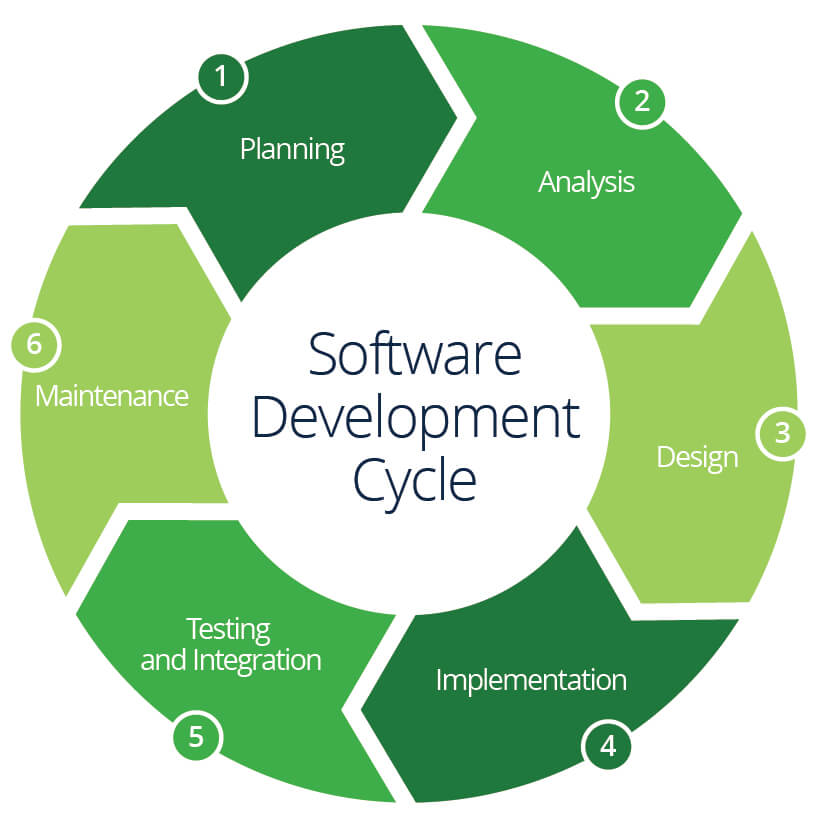
\includegraphics[width=0.4\textwidth]{abb/SDLC}
  \end{center}
  \vspace{-20pt}
  \caption{SDLC}
  \label{fig:sdlc}
  \vspace{-20pt}
\end{wrapfigure}
Mit den entstandenen Testdaten werden erste Methoden entwickelt und damit der System Developement Life Circle (SDLC) in Gang gesetzt (Siehe Abbildung~\ref{fig:sdlc}, S.\pageref{fig:sdlc}). Die Softwareentwicklung durchläuft verschiedene Phasen, die aufeinander aufbauen. Im Laufe der Entwicklung können sich die Phasen im Kreislauf wiederholen, um Änderungen einzuarbeiten und Fehler auszubessern. 



%- Das Projekt läuft über einen Zeitraum von, in dem immer wieder im X und Y Aufnahmen gemacht werden sollen
%- die Testflüge dienten als erste Orientierung, um sich darauf vorbereiten zu können, heraus zu finden welches Equipment notwendig ist und mit den entstandenen Bildern die Softwareentwicklung anzustoßen, aber das ist ein langer Prozess, bis dies tatsächlich beeendet ist.

%Ich nehme mir jetzt diese Testdaten und teste wie mit "einfachen" mitteln das erreicht werden kann. 


% \begin{figure}[htb]
%     \subfigure[15 m]{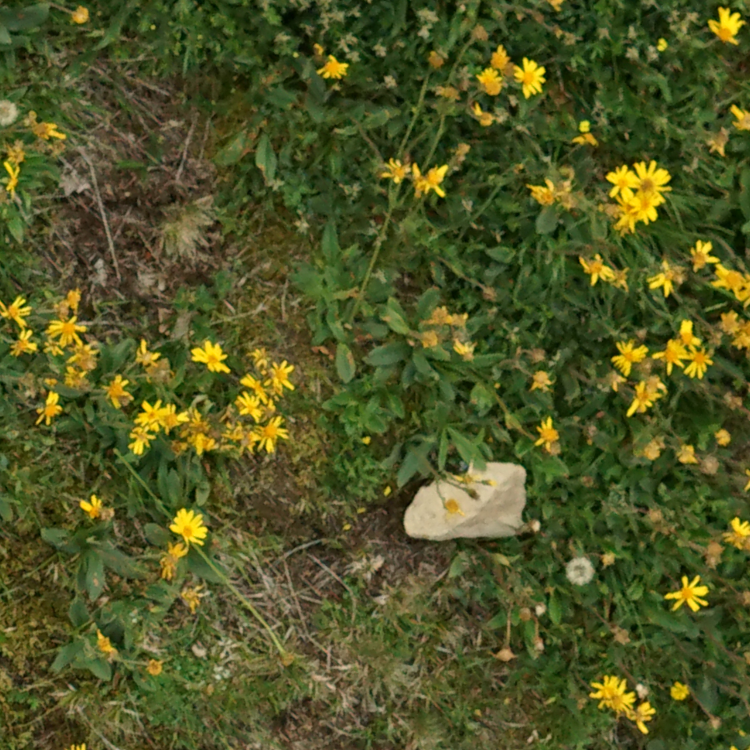
\includegraphics[width=0.24\textwidth]{abb/ergebnisse/gleicheblumen/DSC01525-b}}
%     \subfigure[20 m]{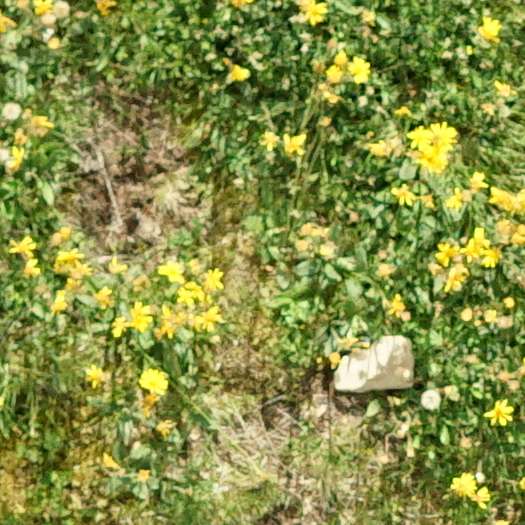
\includegraphics[width=0.24\textwidth]{abb/ergebnisse/gleicheblumen/DSC01298-b}}
%     \subfigure[30 m]{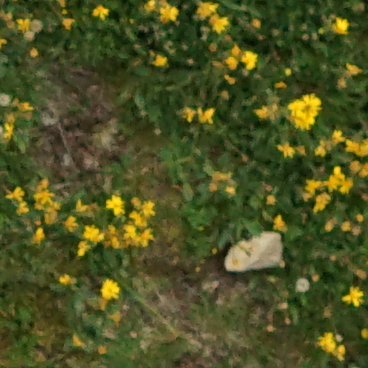
\includegraphics[width=0.24\textwidth]{abb/ergebnisse/gleicheblumen/DSC01757-b}}
%     \subfigure[80 m]{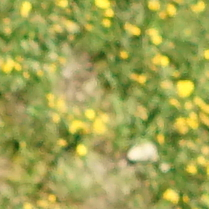
\includegraphics[width=0.24\textwidth]{abb/ergebnisse/gleicheblumen/DSC01959-b}}
% \caption{gleicher Bildausschnitt mit unterschiedlicher Auflösung je nach Flughöhe.}
%   \label{fig:gleicheblumen}
% \end{figure}
%
% Aufnahmenqualität bewerten
%
% \begin{figure}[htb]
%     \subfigure[15m]{\includegraphics[width=0.24\textwidth]{abb/ergebnisse/gleicherausschnitt/DSC01525-a}}
%     \subfigure[20m]{\includegraphics[width=0.24\textwidth]{abb/ergebnisse/gleicherausschnitt/DSC01298-a}}
%     \subfigure[30m]{\includegraphics[width=0.24\textwidth]{abb/ergebnisse/gleicherausschnitt/DSC01757-a}}
%     \subfigure[80m]{\includegraphics[width=0.24\textwidth]{abb/ergebnisse/gleicherausschnitt/DSC01959-a}}
% \caption{Unterschiedlicher Bildausschnitt der Flughöhen bei gleicher Auflösung.}
%   \label{fig:gleicherausschnitt}
% \end{figure}


++++++++++ wissenschaftlicher Kenntnissstand von Monitoring via Drohnen bzw. von automatischer Erkennung und Programmierung 
